\documentclass{article}
\usepackage[utf8]{inputenc}
\usepackage[T1]{fontenc}
\usepackage{graphicx}
\usepackage{hyperref}
\usepackage{geometry}
\geometry{margin=1in}

\title{HELMINTHOLOGY Plate CCLI}
\date{Encyclopaedia Britannica (1771)}

\begin{document}
\maketitle

\section*{Historical source}
\textbf{Entry ID:} \texttt{entry-helminthology-plate-ccli-651} \\
\textbf{Volume ID:} 192692192 \\
\textbf{Character Count:} 79

\subsection*{Extracted Text}
Fig.2.

Fig 1

Fig.2.

Fig.1.

O

Fig.7.

Fig.9.

Fig.9.

Fig.3. Fig.3.

Fig.8.

\subsection*{Matched Wikipedia Article}
\textbf{Title:} Helminthology \\
\textbf{Page ID:} 2203555 \\
\textbf{Revision ID:} 1324313982 \\
\textbf{URL:} \url{https://en.wikipedia.org/wiki/Helminthology}


\section*{Source record}
\begin{itemize}
\item \textbf{Dataset:} \texttt{NationalLibraryOfScotland/encyclopaedia\_britannica\_illustrated}
\item \textbf{Dataset Revision:} \texttt{309f765b1ecc83e0a7f7762e44b4a927a7555443}
\item \textbf{Page ID:} \texttt{britannica:309f765b1ecc83e0a7f7762e44b4a927a7555443:train:651} \\
  \textbf{Filename:} \texttt{page-0651-a4e89a900a40.jpg} \\
  \textbf{Row Index:} 651 \\
  \textbf{SHA256:} \texttt{a4e89a900a4041b9...}
\end{itemize}

\begin{figure}[h]
\centering
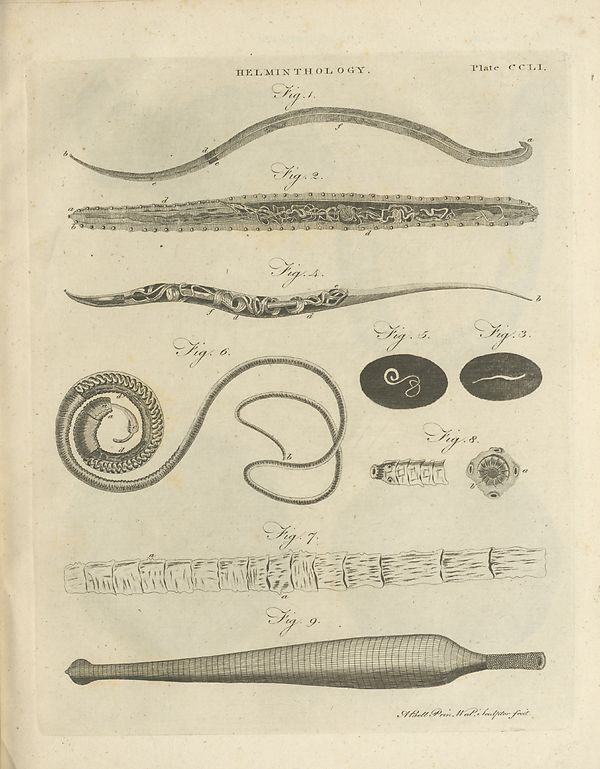
\includegraphics[width=0.85\textwidth]{../scans/page-0651-a4e89a900a40.jpg}
\caption*{Source scan: \texttt{page-0651-a4e89a900a40.jpg}}
\end{figure}

\end{document}
